\section{Validation}\label{sec:validation}

All validation choices were fixed and logged before the first comparison:
\begin{itemize}
\item the matching radii (1, 2 and 5\textdegree, with 2\textdegree{} primary);
\item the statistics (Pearson and Spearman coefficients with bootstrap 95\% confidence intervals, leave-one-site-out ranges, and spatial block bootstrap for GRS);
\item the criterion for claiming an element as validated: Pearson $r>0$ with a 95\% confidence interval excluding zero in both the landing-site and GRS tests.
\end{itemize}
One defect was found after the first comparison and corrected; it is described at the end of this section, and both sets of numbers are reported.

\subsection{Landing sites}\label{sec:sites}
\Cref{tab:sites} lists the returned-soil ratios (average soil compositions; \citealp{Heiken1991}, Table 7.15; \citealp{Basu1998}) and the CLASS weighted means within 2\textdegree{} (\SiteFpMin--\SiteFpMax{} footprints per site).
\begin{itemize}
\item \emph{Mg/Si, 2\textdegree:} $r=\SiteMgTwoR$ (95\% CI \SiteMgTwoCI), leave-one-out range \SiteMgTwoLooLo--\SiteMgTwoLooHi, RMSE \SiteMgTwoRmse, bias \SiteMgTwoBias.
\item \emph{Al/Si, 2\textdegree:} $r=\SiteAlTwoR$ (\SiteAlTwoCI), Spearman $\rho=\SiteAlTwoRho$ ($p=\SiteAlTwoRhoP$), leave-one-out range \SiteAlTwoLooLo--\SiteAlTwoLooHi, RMSE \SiteAlTwoRmse, bias \SiteAlTwoBias.
\item \emph{1\textdegree:} Mg/Si $r=\SiteMgOneR$, Al/Si $r=\SiteAlOneR$.
\item \emph{5\textdegree:} Mg/Si $r=\SiteMgFiveR$, Al/Si $r=\SiteAlFiveR$.
\end{itemize}
The CLASS site means have small statistical errors (\cref{tab:sites}). Their scatter about the soil values is therefore systematic. Footprints of $25\times37$\,km average over terrain far larger than the sampled landing sites, several sites lie on mare--highland contacts (Apollo 15, 16, 17; Luna 20), and the instability of $r$ with radius is what one expects for nine points under these conditions. No element meets the pre-registered landing-site criterion. With $n=9$, a 95\% interval excludes zero only for $r\gtrsim0.67$.

\begin{table}[t]
\centering
\caption{Landing-site validation at 2\textdegree{} radius: returned-soil weight ratios \citep{Heiken1991} and CLASS weighted means $\pm$ standard error.}\label{tab:sites}
\begin{tabular}{lrrrrrr}
\toprule
Site & Lat & Lon & \multicolumn{2}{c}{Mg/Si} & \multicolumn{2}{c}{Al/Si}\\
 & (\textdegree) & (\textdegree E) & soil & CLASS & soil & CLASS\\
\midrule
Apollo 11 & 0.67 & 23.47 & 0.238 & 0.304$\pm$0.005 & 0.365 & 0.596$\pm$0.021\\
Apollo 12 & -3.01 & -23.42 & 0.259 & 0.285$\pm$0.006 & 0.316 & 0.473$\pm$0.014\\
Apollo 14 & -3.65 & -17.47 & 0.252 & 0.327$\pm$0.003 & 0.410 & 0.609$\pm$0.010\\
Apollo 15 & 26.13 & 3.63 & 0.317 & 0.332$\pm$0.007 & 0.353 & 0.162$\pm$0.011\\
Apollo 16 & 8.97 & 15.50 & 0.163 & 0.305$\pm$0.006 & 0.687 & 0.528$\pm$0.023\\
Apollo 17 & 20.19 & 30.77 & 0.311 & 0.321$\pm$0.007 & 0.448 & 0.655$\pm$0.018\\
Luna 16 & -0.68 & 56.30 & 0.272 & 0.308$\pm$0.005 & 0.415 & 0.609$\pm$0.015\\
Luna 20 & 3.53 & 56.55 & 0.280 & 0.297$\pm$0.004 & 0.560 & 0.745$\pm$0.017\\
Luna 24 & 12.71 & 62.20 & 0.276 & 0.307$\pm$0.004 & 0.322 & 0.397$\pm$0.012\\
\bottomrule
\end{tabular}

\end{table}

\subsection{Lunar Prospector GRS}\label{sec:grs}
On the 5\textdegree{} equal-area GRS pixels, all \GrsMgN{} of which contain at least 20 CLASS footprints:
\begin{itemize}
\item \emph{Mg/Si:} $r=\GrsMgR$ (block-bootstrap 95\% CI \GrsMgCI; Spearman $\rho=\GrsMgRho$);
\item \emph{Al/Si:} $r=\GrsAlR$ (\GrsAlCI; $\rho=\GrsAlRho$).
\end{itemize}
Both pass the GRS criterion (\cref{fig:validation}). The correlations are stable under the count-threshold sensitivity test: Mg/Si $r=\GrsMgR$, \GrsMgRMinK, \GrsMgRMinKKK{} and Al/Si $r=\GrsAlR$, \GrsAlRMinK, \GrsAlRMinKKK{} for thresholds of 300, 1000 and 3000 counts (\NMapped, \NMappedMinK{} and \NMappedMinKKK{} spectra). The GRS Mg and Al abundances themselves carry substantial model-dependent uncertainty \citep{Prettyman2006}, so these correlations are lower bounds on the agreement achievable.

\begin{figure}[t]
\centering
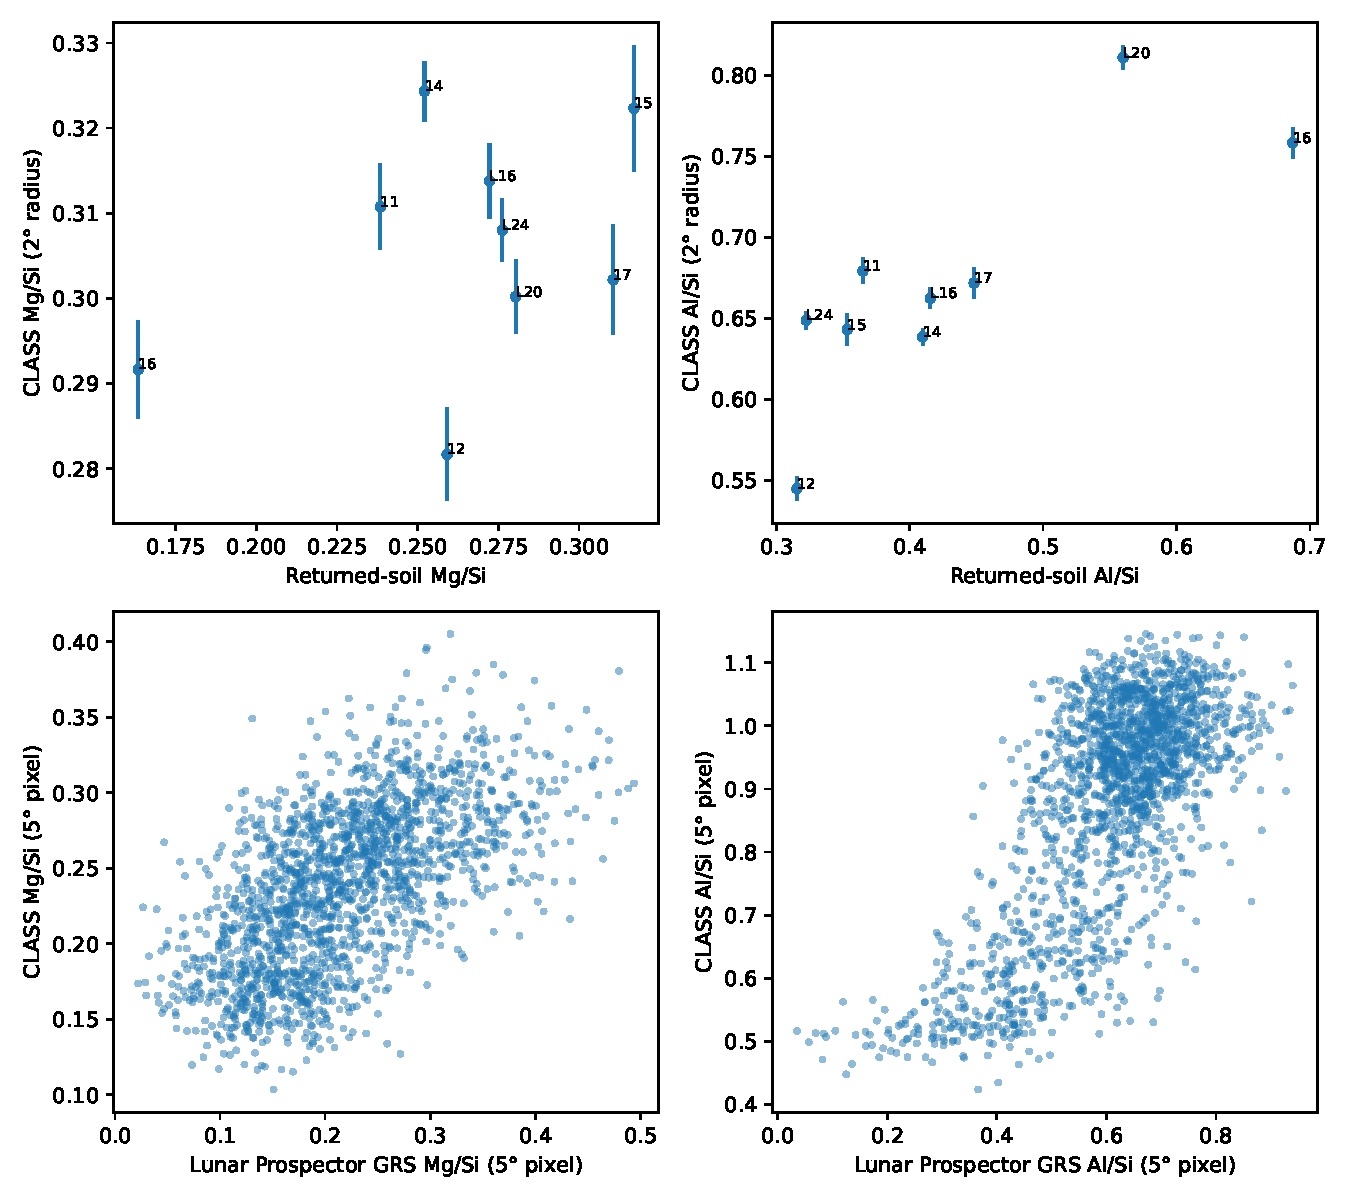
\includegraphics[width=\textwidth]{figures/fig_validation.pdf}
\caption{Top: CLASS ratios within 2\textdegree{} of the landing sites against returned-soil ratios. Bottom: CLASS against Lunar Prospector GRS ratios on 5\textdegree{} equal-area pixels.}\label{fig:validation}
\end{figure}

\subsection{Disclosed post-validation correction}\label{sec:fix}
The first comparison produced a population of Al/Si values near zero. These were 254 fits (0.06\% of the mapping set) in which the instrumental component had absorbed the Al line. Their Al/Si estimates of $\sim10^{-5}$ lay just above the boundary threshold of $10^{-6}$ used to flag pinned parameters. A Fisher-matrix uncertainty is meaningless at a boundary, and theirs had collapsed below $10^{-3}$, so these fits carried 93\% of the total inverse-variance weight. Raising the boundary threshold to $10^{-3}$, below any lunar Mg/Si or Al/Si, removes them.

The pre-correction results were GRS Al/Si $r=\GrsAlRvOne$ (\GrsAlCIvOne), Mg/Si unchanged, and landing-site correlations within 0.02 of the values above. We regard this as a bug fix, not a tuning step, but report it so that readers can judge.

\subsection{What limits the scores?}\label{sec:limits_scores}
Several diagnostics, computed after the pre-registered tests and changing none of them, explain the size of the correlations.

\emph{The landing-site test has little discriminating power at this scale.} Applied to the same nine soil averages, using the 5\textdegree{} pixel containing each site, the Lunar Prospector GRS itself gives $r=\GrsSitesMg$ for Mg/Si and $\GrsSitesAl$ for Al/Si. Site-average soils sample metres to kilometres around each landing point, while orbital pixels average tens to hundreds of kilometres of terrain on mare--highland contacts \citep{Basu1998}. A small or negative $r$ in this test therefore says little about map quality.

\emph{The GRS correlation is bounded by the noise in both data sets.} We split the mapping set into two halves by alternate months, map each half separately, and correlate the two maps. After Spearman--Brown correction, this gives a reliability of the CLASS pixel means of \RelMg{} for Mg/Si and \RelAl{} for Al/Si. The GRS error matrices imply reliabilities of \RelGrsMg{} and \RelGrsAl. The maximum attainable correlation is therefore $\sqrt{\rho_\mathrm{CLASS}\rho_\mathrm{GRS}}=\CeilMg$ for Mg/Si and \CeilAl{} for Al/Si. The observed $r=\GrsMgR$ for Mg/Si is close to its ceiling. For comparison, the earlier processing of the same data gives $r=\OldGrsMg$ and \OldGrsAl{} on the same pixels.

\emph{Al/Si is limited by the instrumental component.} The low split-half reliability of Al/Si comes from month-to-month offsets. In a fixed farside equatorial region, the monthly median Al/Si anticorrelates with the fraction of spectra in which the fitted instrumental amplitude $\gamma$ is non-zero (Spearman $-0.88$). In a few months the free $\gamma$ absorbs part of the lunar Al line.

\paragraph{Post-hoc analyses (labelled as such)} Two variants were examined after validation; neither replaces the pre-registered product.
\begin{itemize}
\item \emph{Weighted median.} Replacing the weighted mean by a weighted median does not help: GRS $r=\MedGrsMg$ (Mg/Si) and \MedGrsAl{} (Al/Si), Al/Si reliability \MedRelAl.
\item \emph{Spectra with $\gamma\approx0$.} The nightside data imply that the instrumental component should be negligible on the dayside (\cref{fig:background}). Restricting the maps to spectra with fitted $\gamma<0.05$ (\GzN{} spectra, \GzPct\% of the mapping set) raises the Al/Si reliability to \GzAlRel. Against GRS, Al/Si then gives $r=\GzAlR$ (\GzAlCI) and Mg/Si $r=\GzMgR$ (\GzMgCI). Against the landing sites at 2\textdegree, Al/Si gives $r=\GzSiteAlR$ (\GzSiteAlCI) and Mg/Si $r=\GzSiteMgR$; the Al/Si site results at 1\textdegree{} and 5\textdegree{} are \GzSiteAlROne{} and \GzSiteAlRFive.
\end{itemize}
The $\gamma$ cut uses a fitted model parameter, not the reference data. It does, however, select spectra after the fact, and its median Al/Si (\GzAlMed) is higher than that of the full set. We therefore present it as evidence that the instrumental-aluminium degeneracy, rather than the fluorescence model, limits Al/Si. A model in which $\gamma$ is fixed to zero on the dayside, specified in advance, is the natural next step. \Cref{fig:posthoc} shows the weighted-median alternative maps.

\begin{figure}[t]
\centering
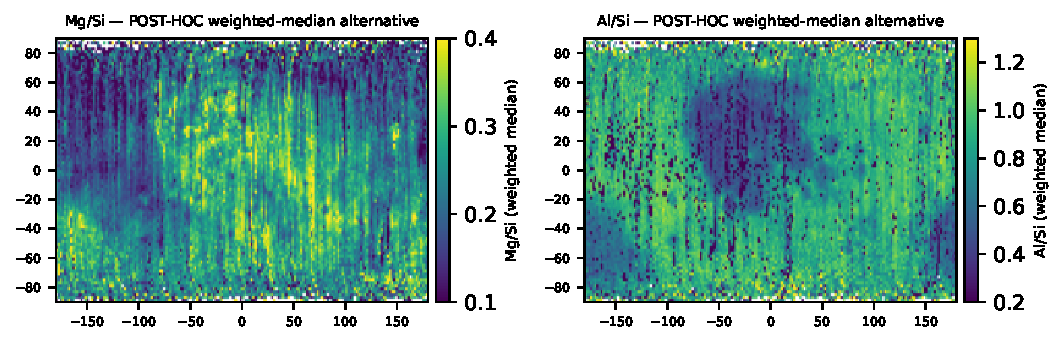
\includegraphics[width=\textwidth]{figures/fig_maps_wmedian_posthoc.pdf}
\caption{\textbf{Post-hoc alternative (not the pre-registered product):} inverse-variance-weighted median of footprint ratios per 2\textdegree{} cell (footprint centres).}\label{fig:posthoc}
\end{figure}

\subsection{Outcome}
Under the pre-registered rule, neither element is claimed as validated: both pass the GRS test, and both fail the nine-site test, which has little statistical power at this footprint size. We therefore present Mg/Si and Al/Si as relative maps whose large-scale pattern agrees with an independent orbital data set, strongly for Mg/Si and moderately for Al/Si, and we make no claim of site-level accuracy. The post-hoc analysis of \cref{sec:limits_scores} indicates that Al/Si can reach a GRS correlation of \GzAlR{} once the instrumental-aluminium degeneracy is controlled.
